
\section{Neural Networks}
\label{sec:neural_networks}
In machine learning research, the goal of a \textit{neural network} is to approximate arbitrary functions. The basic idea of neural networks, so called \textit{perceptrons}, were first introduced by Rosenblatt in \cite{rosenblatt1958perceptron}. While the first neural networks were biologically motivated, neural networks can be interpreted as composition of functions. The relation between these functions forms a directed graph. In this work, we will only cover \textit{feed forward neural networks}. They are called feed forward neural networks because there are no feedback connections: The relation between all functions in the neural network forms an acyclic directed graph. Feed forward networks are an important building block for many machine learning applications. 
\\
More formally, as described in \cite{Goodfellow-et-al-2016}, a feed forward neural network can be described as a model $y = f^*(x, \theta)$, approximating an existing function $y = f(x)$. In this example $x$ is the input, $y$ is the output and $\theta$ are the model parameters which are learned during training. $f$ is the function to approximate and $f^*$ is a composition of many functions with the parameters $\theta$. 
\\
In practice, the functions composing a feed forward neural network are often simply chained, so that their relation graph simply forms a path. In this case, the functional components are called layers. A feed forward neural network of this form with $n$ layers can be written as follows:

\[
y = f^*_n \dots (f^*_2(f^*_1(x, \theta_1), \theta_2) \dots, \theta_n)
\]

For this type of neural network, $f^*_1$ is applied to the input, then $f^*_2$ is applied to the output of $f^*_1$, until the final layer is reached. The output of the final layer is the output of the neural network. Figure \ref{fig:simple_feed_forward_nn} shows a graph based representation of such a neural network. Each node represents a function, arrows represent data flows. 

\begin{minipage}{\linewidth}
	\makebox[\linewidth]{
	\begin{tikzpicture}[x=1.5cm, y=1.5cm, >=stealth]
	
	\node [every neuron] (n0) at (0*1-1,2.5-0) {$x$}; 
	\node [every neuron] (n1) at (1*1-1,2.5-0) {$f^*_1$}; 
	\node [every neuron] (n2) at (2*1-1,2.5-0) {$f^*_2$}; 
	\node [neuron hmissing] (n3) at (3*1-1,2.5-0) {}; 
	\node [every neuron] (n4) at (4*1-1,2.5-0) {$f^*_n$}; 
	\node [every neuron] (n5) at (5*1-1,2.5-0) {$y$}; 
	
	\draw [->] (n0) -- (n1);
	\draw [->] (n1) -- (n2);
	\draw [->] (n2) -- (n3);
	\draw [->] (n3) -- (n4);
	\draw [->] (n4) -- (n5);
	
	\end{tikzpicture}
	}
	\captionof{figure}{Simple graphical interpretation of feed forward neural network}
	\label{fig:simple_feed_forward_nn}
	\hspace{1cm}
\end{minipage}


Even with this simplification, it has been shown that such a feed forward neural network can approximate any function with any desired accuracy. This is called the \textit{universal approximation theorem}, the proof can be found in \cite{hornik1989multilayer}. The caveat is finding the correct function $f^*_n$ to use in each layer and the correct parameters $\theta_n$. Also, finding the function to approximate is non-trivial in the first place. We will discuss these problems in the next sections. 

\subsection{Training Neural Networks}

As with most machine learning approaches, we train the neural  network using by using a \textit{training dataset}, containing a lot of data points sampled from the distribution we seek to approximate. We usually do not want the neural network to excel on the training data set, but rather to perform well on unseen data. This ability is called \textit{generalization}. We can approximate the error on unseen data by testing the neural network on a \textit{test dataset}. The test dataset must never be used for adjusting the neural network parameters, as this will make the test dataset worthless. The situation where a network performs well on the training dataset but worse on the test dataset is called \textit{overfitting}. The network basically memorizes the distribution of the training dataset, but fails to generalize on the test dataset. \\
Given the definition in the past section, we can treat the problem of training a given neural network as finding appropriate parameters $\theta$ to minimize a certain \textit{error function} or \textit{loss function} $E = \mathcal{L}(y)$, where $E$ denotes the error and $y$ the network output. The error $E$ is usually some metric that judges the network performance based on the training data set. The state of the art algorithm for optimizing the parameters of a neural network is called \textit{stochastic gradient descend}, a special application of naive \textit{gradient descend}.
\subsubsection{Naive Gradient Descent}
\label{sec:gradient_descend}
To apply gradient descend, we have to calculate the derivative of the loss function, given a certain input, with respect to a certain parameter $\theta_i$. Since this derivative is multi-dimensional, it is called the \textit{gradient}. Given a feed forward neural network, we can write the error as follows:

\[
E = \mathcal{L}(f^*_n \dots (f^*_2(f^*_1(x, \theta_1), \theta_2) \dots, \theta_n))
\]

Thus, the derivative of the error with respect to a certain weight can be calculated by applying the chain rule.
\[
\frac{\partial E}{\partial \theta_i} = 
	\frac{\partial \mathcal{L}}{\partial y_n}
	\frac{\partial f^*_n}{\partial y_{n - 1}}
	\dots
	\frac{\partial f^*_{i + 2}}{\partial y_i}
	\frac{\partial f^*_i}{\partial \theta_i}
\]

Where $y_k$ is the result of $f^*_k$. \\
We know that the gradient $\frac{\delta E}{\delta \theta_i}$ will become zero in a local minimum, local maximum or saddle point of our error $E$. Since the gradient also gives the direction of the steepest slope, we can simply update our parameters iteratively, until we converge into a local minimum.

\[
	\theta_{i, t+1} = \theta_{i, t} - \epsilon * \frac{\delta E_{t}}{\delta \theta_{i, t}}
\]

In this equation, $t$ denotes the current time and the parameter $\epsilon$ is the so-called learning rate. $\epsilon$ has to be chosen by the designer of the neural network and influences not only the speed of convergence, but also whether the network converges at all. In literature, propagating the error gradient through a neural network is called \textit{backpropagation}. Backpropagation in the context of neural networks was first described in \cite{werbos1974beyond}.

\subsubsection{Stochastic Gradient Descend}

In practice, naive gradient descend does not work well, as described in \cite{wilson2003general}. The reason is that the function we seek to optimize when training a neural network is not convex and might have many local minima. Optimizing iteratively on a stationary error term makes this approach prone to falling into local minima. \\ \\
The state of the art algorithm for training neural networks is called \textit{stochastic gradient descent} (\textit{SGD}), which was first described in a context of neural networks in \cite{bottou1991stochastic}. Stochastic gradient descent introduces two fundamental changes and is. First, we no longer calculate our error term and corresponding gradient for the whole dataset, but for a randomly sampled subset of our data set, which is called a \textit{mini batch}, where the size of the mini batches is a design parameter. Second, we decrease our learning rate while training progresses. According to \cite{Goodfellow-et-al-2016}, iterating on mini batches adds noise to our error term, which in turn offers a regularization effect which was shown to lead to better generalization.
\\ \\
The noise introduced by stochastic gradient descend originates from the fact that we batch our dataset. Even if all batches, if averaged, represent the same distribution as our whole test dataset, each batch has a slightly different distribution. The shape of the loss function, and thus the gradient, changes slightly with each mini batch. This is the main reason why stochastic gradient descend is less prone to get stuck in local minima then naive gradient descend. The noise added by this stochastic process does not go away, even when we reach a global minimum. According to \cite{Goodfellow-et-al-2016}, this is be the main motivation for decreasing the learning rate over time. Furthermore, this property implies that the mini batch size is also an important design choice for achieving good generalization, not only for achieving fast training. 
\\ \\
A disadvantage of stochastic gradient descend is the slower convergence, since we need more steps. This is remedied by the fact that it is easier to calculate the gradient for a small mini batch instead of the whole dataset at once. In practice, we usually shuffle our dataset, split it into mini-batches, and then process each mini batch once. An iteration over all mini batches in the dataset is called an \textit{epoch}. 

\subsubsection{Learning Rates and Learning Rate Scheduling}

With stochastic gradient descend, we choose a separate learning rate $\epsilon_k$ for each epoch $k$. In the scope of this work, we only introduce \textit{exponential decay}, a very simple scheduling algorithm for the learning rate, although numerous other schedulers exist. \\
Exponential starts with a learning rate $k_0$ for the initial batch and multiplies the learning rate by a factor of $0 < p < 1$ after each epoch. 
\[
k_n = k_{n - 1} * p
\]
A variant of exponential decay keeps the learning rate constant for a number epochs, until the improvement of error measured on the test dataset falls below a certain threshold $t$. This variant is called \textit{newbob}. Newbob scheduling is widely used by the speech recognition community. It was first introduced in \cite{berkely2000newbob}.

\subsubsection{Momentum}
\label{sec:momentum}

\textit{Momentum} is another technique that was shown to avoid local minima. When using momentum, we do not apply the gradient directly to our model, but rather use a linear combination of the gradient of the last batches. There are multiple versions to achieve momentum when using stochastic gradient descend. This work uses the notation introduced in \ref{polyak1964some} and throughly analyzed in the context of deep learning in \ref{sutskever2013importance}:
\begin{align*}
\upsilon_{i, t+1} &= \upsilon_{i, t} * \rho + \epsilon * \frac{\delta E_{t}}{\delta \theta_{i, t}} \\
\theta_{i, t+1} &= \theta_{i, t} - \upsilon_{i, t+1}
\end{align*}
Here, $\upsilon$ is called the \textit{velocity}, it is a linear combination of the last velocity and the current gradient. $\rho$ is the term defining the momentum. It defines how much of the velocity is added to the current gradient. All other variables are defined as in section \ref{sec:gradient_descend}.
\subsection{Neural Network Architectures}

In practice, neural network layers are often formed by combining an affine transformation with a non-linear function. Since affine transformations of data vectors can be interpreted as matrix-vector multiplications, we can write a layer function in the following way, where $x_k$ is the input vector for $k$th layer, $W_k$ is the matrix defining the affine transformation of the $k$th layer, and $\varphi$ is a non-linear activation function of layer $k$.
\[
f^*_k(x_k) = \varphi_k(W_k x_k)  
\]
The count of layers, as well as the size of each $W_k$ are design decisions and depend on the task. We call the count of layers \textit{depth} of a neural network, and count of rows in $W_k$ the \textit{width} of layer $k$. The contents of $W_k$, called the \textit{weights} of layer $k$, are the trainable parameters $\theta$ for models of this form.
\pagebreak
\subsubsection{Activation Functions}

Non-linear activation functions, or simply \textit{activation functions}, can be roughly classified into two groups: Activation functions which are applied element-wise and thus do not change the dimension of the data, as well as activation functions which are applied on groups of elements of the input vector and change the dimension. The latter case is commonly fund with so called pooling functions. The choice of the activation function $\varphi$ has significant impact on the performance of a neural network and has been subject to many bodies of research, as summarized in \cite{thoma2017analysis}. In this work, we will only discuss the \textit{ReLU}, \textit{p-norm} and \textit{softmax} activation functions. 

\subsubsection*{Rectified Linear Unit (ReLU)}
% ReLU
\begin{minipage}{0.45\textwidth}
	\[\varphi^{ReLU}(x) = \begin{cases}
	0 & x < 0 \\
	x & x \geq 0
	\end{cases}\]
	First introduced in \cite{krizhevsky2012imagenet}, ReLU nonlinearities have proven successful in practice. The computation of ReLU nonlinearity is cheap, also the gradient never saturates for positive values of $x$. For negative values, the gradient is zero, which can be a disadvantage.  
\end{minipage}
\hfill
\begin{minipage}{0.45\textwidth}
\begin{tikzpicture}[baseline=(current bounding box)]
\begin{axis}[xmin=-2,xmax=2,ymin=-2,ymax=2,axis lines = middle,xlabel = $x$,ylabel = $\varphi^{ReLu}(x)$,clip = false]
\addplot+[mark=none,blue,domain=-2:0] {0};
\addplot+[mark=none,blue,domain=0:2] {x};
\end{axis}
\end{tikzpicture} 
\captionof{figure}{The ReLU function.}
\end{minipage}
% L2 Pooling

\subsubsection*{P-norm}
\begin{minipage}{0.45\textwidth}
	\[\varphi^{Lp}(X) = \sqrt[p]{ \sum_{x \in X}{x^p} } \] 
	The p-norm nonlinearity was described by \cite{zhang2014improving}. This nonlinearity operates on a set $X$ of input elements and reduces them to one. The group size as well as the $p$ are a design parameter. For a fixed $p$ of $2$, the p-norm is also called \text{L2 pooling}.
\end{minipage}
\hfill
\begin{minipage}{0.45\textwidth}
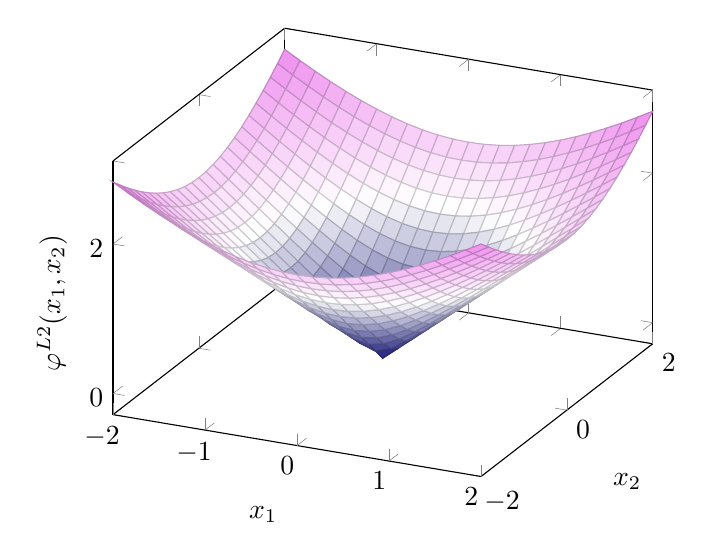
\begin{tikzpicture}[baseline=(current bounding box)]
\begin{axis}[xmin=-2,xmax=2,ymin=-2,ymax=2,xlabel = $x_1$,ylabel = $x_2$,zlabel = $\varphi^{L2}({x_1, x_2})$,colormap/violet,clip = false]
\addplot3[surf,samples=25, domain=-2:2]
{sqrt(x * x + y * y)};
\end{axis}
\end{tikzpicture}
\captionof{figure}{Example of p-norm with $p = 2$ and and an input group containing two values}
\end{minipage}

\subsubsection*{Softmax}
\begin{minipage}{0.45\textwidth}
	\[\varphi^{softmax}_{\tau}(X)_i = \frac{e^\frac{x_i}{\tau}}{ \sum_{x_j \in X} e^\frac{x_j}{\tau} } \]
	The softmax activation is defined as an operation over the whole input, but does not reduce the dimension. It maps all output values to a space between $0$ and $1$, preserves the rank of each output and also guarantees that the sum over all outputs is exactly $1$. Therefore it produces a valid probability distribution and is usually used for the last layer of a neural network for classification problems. The term $\tau$ is called the softmax temperature. It can be used to change the contrast of the distribution produced by the softmax activation. A higher temperature $\tau$ will lead to a distribution more smooth. A lower $\tau$ will lead to a more sharp distribution, that concentrates a higher probability at the maximum value. 
\end{minipage}
\hfill
\begin{minipage}{0.45\textwidth}
	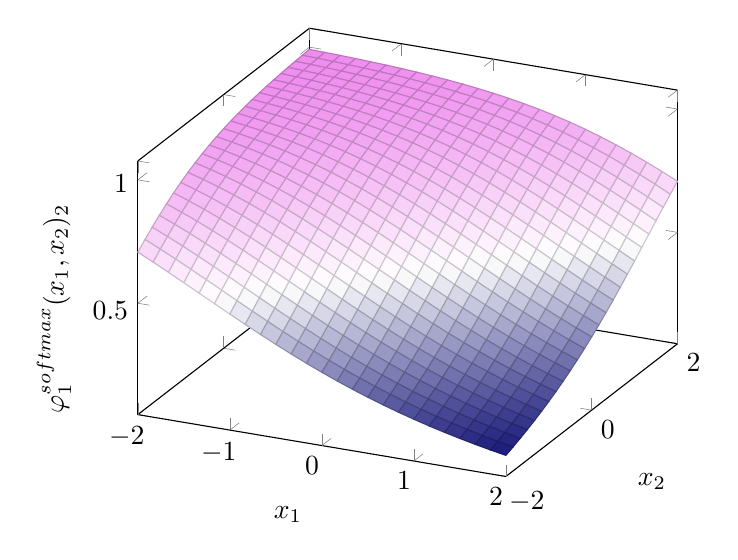
\begin{tikzpicture}[baseline=(current bounding box)]
	\begin{axis}[xmin=-2,xmax=2,ymin=-2,ymax=2,xlabel = $x_1$,ylabel = $x_2$,zlabel = $\varphi^{softmax}_{1}({x_1, x_2})_2$,colormap/violet,clip = false]
	\addplot3[surf,samples=25, domain=-2:2]
	{sqrt(e^y / (e^x + e^y) )};
	\end{axis}
	\end{tikzpicture}
	\captionof{figure}{Example of a vanilla softmax ($\tau = 1$) for an input vector containing two values}
	\vspace{0.5cm}
	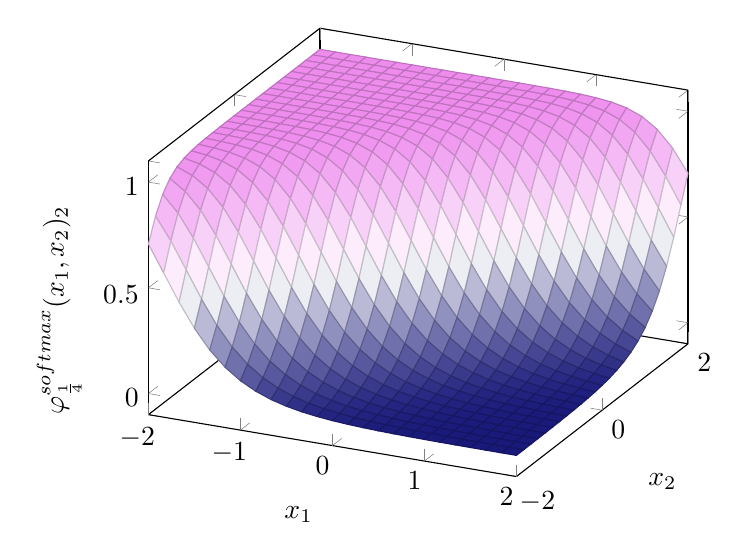
\begin{tikzpicture}[baseline=(current bounding box)]
	\begin{axis}[xmin=-2,xmax=2,ymin=-2,ymax=2,xlabel = $x_1$,ylabel = $x_2$,zlabel = $\varphi^{softmax}_{\frac{1}{4}}({x_1, x_2})_2$,colormap/violet,clip = false]
	\addplot3[surf,samples=25, domain=-2:2]
	{sqrt(e^(y * 4) / (e^(x * 4) + e^(y * 4)) )};
	\end{axis}
	\end{tikzpicture}
	\captionof{figure}{Example of a softmax with adjusted temperature ($\tau = \frac{1}{4}$) for an input vector containing two values}
\end{minipage}

\subsubsection{Batch Normalization}
Several different forms of batch normalization exist. In this work, we only consider the concept introduced in \cite{IoffeS15}, which can be formulated as follows: 
\[
y = \frac{x - E[x]}{\sqrt{Var[x] + \epsilon}}
\]
Here, $Var[x]$ is the variance of our input vector $x$, $E[x]$ is the expected value of $x$ and $\epsilon$ is a small constant to avoid division by zero. The normalization is not applied on a single value of $x$, but rather on a whole batch when using stochastic gradient descend. The motivation behind batch normalization is to fix the distribution of activations within the network, where the mean is fixed to $0$ and the variance is fixed to $1$. This makes it easier to use nonlinearities which saturate for very large or very small activations. 

\subsection{The Cross Entropy Loss Function}

There exist numerous loss functions for neural networks. Technically, any metric can be used as loss function, although loss functions do not necessarily have to be metrics. One of the most widely loss functions for classification tasks is the \textit{cross entropy} (\textit{CE}) function. For two  probability vectors $p$ and $q$, the cross entropy can be written as follows:

\begin{align}
H(p, q) = - \sum_{x} p(x) \log q(x)
\label{eq:cross_entropy_loss}
\end{align}

The cross entropy loss function has several important properties. First, it minimizes the so called \textit{Kullback-Leibler} (\textit{KL}) divergence. The Kullback-Leibler divergence measures the distance of two probability distributions and was introduced in \cite{kullback1951information}. The Kullback-Leibler divergence is equal to zero if, and only if, the two given distributions are also equal. For two probability vectors $p$ and $q$, it can be written in the following way:

\[
D_{KL}(p, q) = -\sum_{x} p(x) \log \frac{p(x)}{q(x)}
\]

To show the connection between the cross entropy and the Kullback-Leibler divergence, we first assume that $q$ is the distribution we seek to optimize. Thus $p$ can be thought of as an example from our training dataset, or in other words, the distribution we seek to match. Therefore, $p$, can be assumed to be constant. We can write the Kullback-Leibler divergence as follows: 

\begin{align*}
D_{KL}(p, q) &= - \sum_{x} p(x) \left[ \log p(x) - \log q(x) \right] \\
& = - \sum_{x} p(x) \log p(x) -\sum_{x} p(x) \log q(x)
\end{align*}

Since we are not interested minimizing the distribution $p$, we can drop the first sum, and thus receive the cross entropy loss as in equation \ref{eq:cross_entropy_loss}. 
\subsection{Cross Entropy Loss for Classification}
\label{sec:ce_loss}
When training neural networks, we often deal with classification problems. In this case, we seek to assign a single class to a given input sample, our target probability $p$ has exactly one element which is one, all other elements are zero. In this case, the cross entropy loss can be simplified to the so called \textit{negative log likelihood loss}, where $i$ is the index of the correct class in $p$. 

\begin{align}
D_{NLLL}(i, q) = -\log q(i)
\label{eq:nlll}
\end{align}

It has to be noted that this loss functions all operate on probability vectors: All elements have to be between $0$ and $1$ and sum to unity. Therefore, a softmax activation function is usually applied before calculating the loss. \\ \\
It can further be shown that training using a cross entropy loss function trains the network to predict \textit{posteriori} probabilities \cite{richard1991neural}. Formally, given an network input $x$ and a class $c_i$, the network will predict $p(c_i|x)$. Since posteriors are inherently biased towards more frequent classes, we might want to estimate the likelihood $p(x|c_i)$ instead, depending on our use case. With bayes' theorem, we can write the posterior depending on the likelihood. 
\[
p(c_i|x) = \frac{p(x|c_i) p(c_i)}{p(x)}
\]
We now assume $p(x)$ to be equal for all $x$ and solve the equation for the likelihood:
\[
p(x|c_i) = \frac{p(c_i|x)}{p(c_i)}
\]
The probability of observing a certain class $p(c_i)$ is called a \textit{prior}. The prior can be estimated from the training data, or from the network output given a random sample of the training data set. Using the likelihood instead of the prior is especially important when the examples in the training set are highly unbalanced with regard of one or more classes. 
